\section{Results}

A comparison of the radionuclide production between a cell rnucs, meshed rnucs, and geometry split rnucs  for Toy Problem 
I and Toy problem II are shown 
in Figures \ref{1prod_cell_2x} and \ref{2prod_cell_2x} respectively. \\
\begin{figure}[h]
 \begin{centering}
 \centering
 \begin{subfigure}[b]{.45\textwidth}
 \frame{\includegraphics[width=0.95\linewidth,height=5cm]{../figs/toy_p1/1prod_rate_cell_2x.png}}
 \caption{Toy problem I }
 \label{1prod_cell_2x}
 \end{subfigure}
 \hspace{0.05cm}
 %
 \begin{subfigure}[b]{.45\textwidth}
 \centering
 \frame{\includegraphics[width=.95\linewidth,height=5cm]{../figs/toy_p2/2prod_rate_cell_2x.png}}
 \caption{Toy problem II}
 \label{2prod_cell_2x}
 \end{subfigure}
 \caption{Radionuclide production for cell, meshed and split geometries}
 \label{prod_cell_2x}
 \end{centering}
\end{figure}

Figures \ref{1spect_cell_2x} and \ref{2spect_cell_2x} show a similar comparison for the photon spectrum.  \\

\begin{figure}[h]
 \begin{centering}
 \centering
 \begin{subfigure}[b]{.45\textwidth}
 \frame{\includegraphics[width=0.95\linewidth,height=5cm]{../figs/toy_p1/1spectrum_cell_2x_t32.png}}
 \caption{Toy problem I }
 \label{1spect_cell_2x}
 \end{subfigure}
 \hspace{0.05cm}
 %
 \begin{subfigure}[b]{.45\textwidth}
 \centering
 \frame{\includegraphics[width=.95\linewidth,height=5cm]{../figs/toy_p2/2spectrum_cell_2x_t32.png}}
 \caption{Toy problem II}
 \label{2spect_cell_2x}
 \end{subfigure}
 \caption{Photon Spectrum at 1hr after shutdown }
 \label{spect_cell_2x}
 \end{centering}
\end{figure}

Figures \ref{prod_cell_2x} and \ref{spect_cell_2x} suggest that the splitting the geometries 
differs the most from the original rnucs workflow. In this particular case, splitting the geometry 
into 8 equal parts for Toy problem II required material mixing. This is likely to show in the large 
discrepancy between the cell case and the split case. 


Another important comparison is that of the cell rnucs with the progression of the mesh rnucs. 
Figure \ref{voxels} shows the order of the voxels used in Figure \ref{spect_cell_2x_byV}. 


\begin{figure}[h]
\begin{centering}
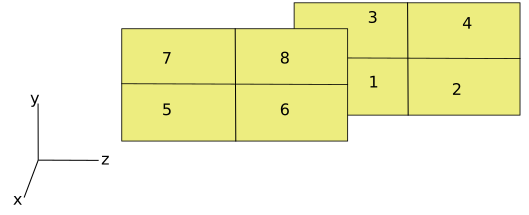
\includegraphics[width=0.60\linewidth]{../figs/voxels.png}
\caption{Voxel configuration}
\label{voxels}
\end{centering}
\end{figure}

\begin{figure}[h]
 \begin{centering}
 \centering
 \begin{subfigure}[b]{.45\textwidth}
 \frame{\includegraphics[width=0.95\linewidth,height=5cm]{../figs/toy_p1/1spectrum_cell_2x_byV_t32.png}}
 \caption{Toy problem I }
 \label{1spect_cell_2x_byV}
 \end{subfigure}
 \hspace{0.05cm}
 %
 \begin{subfigure}[b]{.45\textwidth}
 \centering
 \frame{\includegraphics[width=.95\linewidth,height=5cm]{../figs/toy_p2/2spectrum_cell_2x_byV_t32.png}}
 \caption{Toy problem II}
 \label{2spect_cell_2x_byV}
 \end{subfigure}
 \caption{Photon Spectrum at 1hr after shutdown for each voxel in a 2x2x2 mesh}
 \label{spect_cell_2x_byV}
 \end{centering}
\end{figure}

In Figure \ref{spect_cell_2x_byV} there are three distinct set of the lines, the 
first one is the one for the cell, the second set belong to voxels 1, 3, 5, and 7, and the 
last group belongs to voxels 2, 4, 6, and 8. Voxels 1, 3, 5, and 7 have greater photon emission 
than the voxels 2, 4, 6, and 8. This is expected as the source is to the left of the geometry. 
Having a mesh gives more spatial definition which is useful for large geometric cells. 
